\FloatBarrier
\section{Frozen Checkpoint and Configuration}\label{app:manifest}

All results of \cref{sec:evaluation} come from one checkpoint frozen before the first run. Table~\ref{tab:manifest} lists the hashes recorded in its manifest; the local copies of the controller, trainer, harness, calibration files, and simulator were checked against them when this paper's tables were generated. Every number in the paper is produced by one script from the run directories and the frozen files, not typed by hand.

\begin{table}[!htbp]
\caption{Hashes of the frozen checkpoint (first 16 hexadecimal digits of SHA-256).}
\label{tab:manifest}
\centering\small
% generated by code/specsched/paper_assets.py -- do not edit by hand
\begin{tabular}{@{}ll@{}}
\toprule
Component & SHA-256 (first 16 hex digits)\\
\midrule
\texttt{controller.py} & \texttt{0c526960ecb25143} \\
\texttt{train\_head.py} & \texttt{cc224db0c6b40c81} \\
\texttt{hotswap\_run.py} & \texttt{866e1159bda44604} \\
\texttt{livetap.py} & \texttt{719538857da7d833} \\
\texttt{sched/model.json} & \texttt{18c3723adbe9b858} \\
\texttt{sched/model\_m2.json} & \texttt{5c9fa2d452ca7156} \\
\texttt{sched/sim.py} & \texttt{451c5673bbb4c7a4} \\
\texttt{vllm/v1/worker/gpu\_model\_runner.py} (patched) & \texttt{08c3099b3f725380} \\
\texttt{vllm/v1/worker/gpu\_worker.py} (patched) & \texttt{ca3add781f3ab162} \\
\texttt{vllm/v1/core/sched/scheduler.py} (patched) & \texttt{a8670d8b381dde71} \\
\texttt{vllm/v1/engine/core.py} (patched) & \texttt{e9353a6d8cd9cfe4} \\
\texttt{vllm/v1/spec\_decode/live\_tap.py} (patched) & \texttt{cae550fdf2ad39d1} \\
\texttt{vllm/v1/worker/gpu/model\_runner.py} (patched) & \texttt{ade8b970f18d7533} \\
Drafter \texttt{qwen3-8b-eagle3} & \texttt{048b9c4ada5fc26a} \\
Drafter \texttt{qwen3-a3b-eagle3} & \texttt{dc6373b07e6eb6c1} \\
Target weights, Qwen3-8B / Qwen3-30B-A3B & \texttt{f7c4eadfbbf52247} / \texttt{2850ddb3bf7aecad} \\
Software & torch 2.13.0, transformers 5.15.1, triton 3.7.1, vllm 0.27.1 \\
\bottomrule
\end{tabular}

\end{table}

\paragraph{Engine.} vLLM 0.27.1 (V1 engine), one H100 GPU per run, \texttt{max\_num\_seqs} 256, maximum model length 4{,}096, prefix caching disabled, greedy decoding, outputs of at most 512 tokens with natural stopping. GPU memory utilization is \nv{util.prod} for \pol{Production} and 0.90 minus the trainer's reserve for all other policies (\nv{util.m1} for Qwen3-8B, \nv{util.m2} for the MoE target). EAGLE-3 drafters with $k{=}3$, auxiliary target layers $(2,18,33)$ for Qwen3-8B and $(2,24,45)$ for Qwen3-30B-A3B, and a 32k draft vocabulary. The feature export uses a 4\,GB shared-memory ring and samples every step.

\paragraph{Trainer.} Cross-entropy on the target's next tokens over the draft vocabulary; AdamW with learning rate $5\times10^{-5}$, betas $(0.9,0.95)$, no weight decay, 10 warm-up steps, and gradient clipping at 1.0; about 4{,}096 tokens per step and at most 2{,}048 tokens per sequence; a last-in-first-out buffer of at most 600k tokens with a 60\,s age limit; duty cycle by sleeping $(1-d)/d$ times the step time. The trainer's seed is the repetition index.

\FloatBarrier
\section{Workloads and Calibration}\label{app:calibration}

\subsection{Workloads}\label{app:workloads}

Table~\ref{tab:workloads} describes the domains. For calibration, each domain was deduplicated and shuffled, and the target generated greedy outputs for 3{,}200 training, 300 evaluation, and 300 reserve prompts. The prompts of phase B in the evaluation come from separate pools of unique prompts that exclude every calibration prompt (16{,}222 code and 44{,}776 Chinese prompts); phases A1 and A2 use two disjoint sets of 200 chat prompts per repetition.

\begin{table}[!htbp]
\caption{Domains. Token counts are means over the target's greedy outputs (Qwen3-8B); \emph{Truncated} is the share of outputs that hit the 512-token limit; \emph{Coverage} is the share of target output tokens inside the 32k draft vocabulary. MATH-500 is used only for the long-output sweep, with thinking enabled and outputs of up to 4{,}096 tokens.}
\label{tab:workloads}
\centering\footnotesize\setlength{\tabcolsep}{4pt}
% generated by code/specsched/paper_assets.py -- do not edit by hand
\begin{tabularx}{\linewidth}{@{}l>{\raggedright\arraybackslash}Xrrrrr@{}}
\toprule
Domain & Source & Prompts & Prompt tok. & Output tok. & Truncated & Coverage\\
\midrule
Chat & UltraChat 200k \citep{ding2023ultrachat} & 3{,}800 & 109 & 439 & 73.7\% & 95.8\% \\
SQL & sql-create-context \citep{sqlcreatecontext} & 3{,}800 & 68 & 27 & 0.0\% & 91.5\% \\
Code & CodeAlpaca-20k \citep{codealpaca} & 3{,}800 & 38 & 275 & 15.5\% & 97.6\% \\
Chinese & alpaca-gpt4-zh \citep{peng2023gpt4instruct} & 3{,}800 & 25 & 314 & 36.8\% & 42.6\% \\
Function calling & Glaive function calling v2 \citep{glaivefc} & 3{,}800 & 219 & 30 & 0.0\% & 91.3\% \\
MATH-500 & MATH-500 \citep{lightman2023verify} & 500 & 98 & 3{,}324 & -- & -- \\
\bottomrule
\end{tabularx}

\end{table}

\FloatBarrier
\subsection{Calibration measurements}

The calibration consists of four measurements, all on one H100 with vLLM 0.27.1 and taken before the freeze; the frozen calibration files store the fits derived from them.

\paragraph{Load sweep.} Closed-loop benchmark at fixed concurrency, plain decoding versus factory-drafter speculation (Table~\ref{tab:loadsweep}). Step times from this sweep give $T_{\mathrm{base}}(C)$ and $T_{\mathrm{spec}}(C)$.

\paragraph{Training interference.} The same benchmark with a trainer on the GPU at duty cycles 0.1, 0.25, 0.5, and 1 (Table~\ref{tab:duty}); $\kappa(C)$ is fitted from it.

\paragraph{Learning curves.} One pass over the 3{,}200 training prompts of each domain in arrival order, exporting drafters after 100, 200, \dots{}, 3{,}200 requests and measuring their acceptance on the evaluation prompts (Table~\ref{tab:learning}).

\paragraph{Frontier.} Throughput of plain decoding and of three or four drafter checkpoints per domain at six loads (Figure~\ref{fig:frontier}); per load, a line through the (acceptance, ratio) points gives $\alpha_\ell(C)$ and $\beta_\ell(C)$ (Table~\ref{tab:frontier}).

\begin{table}[!htbp]
\caption{Load sweep with factory drafters (closed loop, one H100).}
\label{tab:loadsweep}
\centering\small
% generated by code/specsched/paper_assets.py -- do not edit by hand
\begin{tabular}{@{}lrrcc@{}}
\toprule
Concurrency & Plain tok/s & Spec.\ tok/s & Acceptance & Spec./plain\\
\midrule
\multicolumn{5}{@{}l}{\textit{Qwen3-8B, short outputs (chat)}}\\
$C{=}1$ & 120 & 191 & 1.89 & 1.59$\times$ \\
$C{=}2$ & 230 & 365 & 1.88 & 1.59$\times$ \\
$C{=}4$ & 451 & 688 & 1.87 & 1.52$\times$ \\
$C{=}8$ & 785 & 1{,}258 & 1.89 & 1.60$\times$ \\
$C{=}16$ & 1{,}602 & 2{,}435 & 1.89 & 1.52$\times$ \\
$C{=}32$ & 3{,}064 & 4{,}533 & 1.89 & 1.48$\times$ \\
$C{=}64$ & 5{,}454 & 7{,}695 & 1.91 & 1.41$\times$ \\
$C{=}128$ & 9{,}306 & 10{,}675 & 1.90 & 1.15$\times$ \\
$C{=}256$ & 13{,}758 & 11{,}887 & 1.90 & 0.86$\times$ \\
\multicolumn{5}{@{}l}{\textit{Qwen3-8B, long outputs (MATH-500, thinking)}}\\
$C{=}1$ & 118 & 209 & 2.08 & 1.76$\times$ \\
$C{=}4$ & 441 & 745 & 2.11 & 1.69$\times$ \\
$C{=}16$ & 1{,}307 & 2{,}246 & 2.13 & 1.72$\times$ \\
$C{=}64$ & 3{,}405 & 5{,}907 & 2.12 & 1.74$\times$ \\
$C{=}96$ & 4{,}133 & 7{,}060 & 2.12 & 1.71$\times$ \\
\multicolumn{5}{@{}l}{\textit{Qwen3-30B-A3B, short outputs (chat)}}\\
$C{=}1$ & 188 & 217 & 2.02 & 1.15$\times$ \\
$C{=}2$ & 287 & 353 & 2.02 & 1.23$\times$ \\
$C{=}4$ & 392 & 519 & 2.05 & 1.33$\times$ \\
$C{=}8$ & 568 & 769 & 2.02 & 1.35$\times$ \\
$C{=}16$ & 854 & 1{,}265 & 2.04 & 1.48$\times$ \\
$C{=}32$ & 1{,}381 & 2{,}182 & 2.04 & 1.58$\times$ \\
$C{=}64$ & 2{,}293 & 3{,}800 & 2.05 & 1.66$\times$ \\
$C{=}128$ & 3{,}889 & 6{,}356 & 2.04 & 1.63$\times$ \\
$C{=}256$ & 6{,}651 & 9{,}963 & 2.04 & 1.50$\times$ \\
\bottomrule
\end{tabular}

\end{table}

\begin{table}[!htbp]
\caption{Training interference: Qwen3-8B, short outputs, speculation on; throughput retained and p99 TPOT change relative to the same load without a trainer.}
\label{tab:duty}
\centering\small
% generated by code/specsched/paper_assets.py -- do not edit by hand
\begin{tabular}{@{}crrrrrrrr@{}}
\toprule
& \multicolumn{4}{c}{Throughput retained (\%)} & \multicolumn{4}{c}{p99 TPOT change (\%)}\\
\cmidrule(lr){2-5}\cmidrule(l){6-9}
Duty $d$ & $C{=}1$ & $C{=}4$ & $C{=}16$ & $C{=}64$ & $C{=}1$ & $C{=}4$ & $C{=}16$ & $C{=}64$\\
\midrule
0.1 & 97.5 & 98.3 & 98.6 & 95.7 & $+4$ & $+3$ & $-5$ & $+5$ \\
0.25 & 90.6 & 90.9 & 91.0 & 87.1 & $+10$ & $+11$ & $+12$ & $+14$ \\
0.5 & 77.8 & 76.1 & 75.7 & 70.6 & $+37$ & $+31$ & $+24$ & $+42$ \\
1 & 50.2 & 48.7 & 45.2 & 39.1 & $+103$ & $+103$ & $+133$ & $+161$ \\
\bottomrule
\end{tabular}

\end{table}

\begin{table}[!htbp]
\caption{Acceptance length after learning online from $N$ requests (one pass, arrival order; measured on held-out evaluation prompts of the same domain). The ceiling $\amax_\ell$ is the row maximum.}
\label{tab:learning}
\centering\small
% generated by code/specsched/paper_assets.py -- do not edit by hand
\begin{tabular}{@{}lcccccccc@{}}
\toprule
Domain & $N{=}0$ & $N{=}100$ & $N{=}200$ & $N{=}400$ & $N{=}800$ & $N{=}1600$ & $N{=}3200$ & Coverage\\
\midrule
8B SQL & 1.88 & 2.11 & 2.31 & 2.45 & 2.50 & 2.57 & 2.63 & 91.5\% \\
8B code & 2.12 & 2.46 & 2.54 & 2.60 & 2.65 & 2.69 & 2.72 & 97.6\% \\
8B Chinese & 1.21 & 1.26 & 1.32 & 1.37 & 1.41 & 1.43 & 1.45 & 42.6\% \\
8B function calling & 2.27 & 2.74 & 2.79 & 2.70 & 2.67 & 2.52 & 2.52 & 91.3\% \\
MoE code & 2.62 & 2.74 & 2.82 & 2.89 & 2.92 & 2.96 & 2.99 & -- \\
\bottomrule
\end{tabular}

\end{table}

\begin{table}[!htbp]
\caption{Break-even acceptance $a^{*}_\ell(C)$ from the linear frontier fit, and the largest absolute residual of the fit over all loads.}
\label{tab:frontier}
\centering\small
% generated by code/specsched/paper_assets.py -- do not edit by hand
\begin{tabular}{@{}lccccccc@{}}
\toprule
Domain & $C{=}1$ & $C{=}4$ & $C{=}16$ & $C{=}64$ & $C{=}128$ & $C{=}256$ & Max.\ residual\\
\midrule
8B code & 1.08 & 1.18 & 1.11 & 1.11 & 1.61 & 2.29 & 0.031 \\
8B SQL & 1.08 & 1.01 & 1.08 & 1.42 & 1.74 & 2.45 & 0.082 \\
8B Chinese & 1.21 & 1.22 & 1.23 & 1.32 & 1.62 & 2.28 & 0.013 \\
MoE code & 1.89 & 1.46 & 1.06 & 0.98 & 1.07 & 1.27 & 0.017 \\
\bottomrule
\end{tabular}

\end{table}

\begin{figure}[!htbp]
\centering
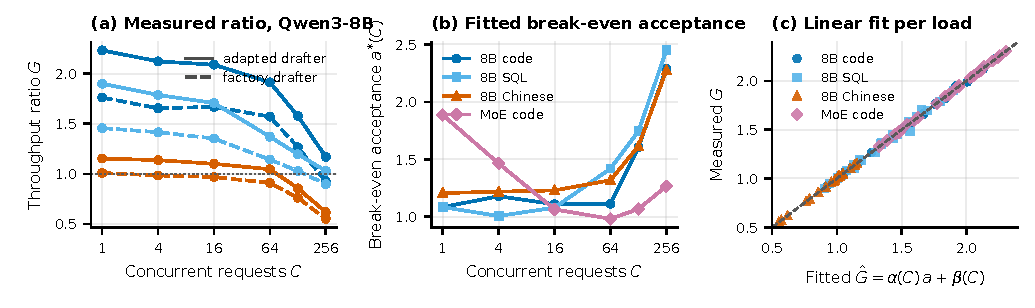
\includegraphics[width=\linewidth]{figures/fig3_frontier.pdf}
\caption{Profitability frontier. (a) Measured speculative over plain throughput for factory (dashed) and adapted (solid) Qwen3-8B drafters; colors as in (b). (b) Fitted break-even acceptance per load. (c) Linear fit versus measurement for all domains and loads.}
\label{fig:frontier}
\end{figure}

\paragraph{Output-length protocol.} Saturated throughput depends on how outputs end (Table~\ref{tab:protocol}). In a batch of 600 requests submitted at once, natural stopping mixes a long drain phase at low concurrency, where speculation is favourable; forcing every output to 256 tokens removes it, and the adapted code drafter then stays below plain decoding. The closed-loop evaluation uses natural stopping, as production traffic does.

\begin{table}[!htbp]
\caption{Code domain, Qwen3-8B: speculative over plain throughput for 600 requests submitted at once, with natural stopping versus outputs forced to 256 tokens.}
\label{tab:protocol}
\centering\small
% generated by code/specsched/paper_assets.py -- do not edit by hand
\begin{tabular}{@{}lccc@{}}
\toprule
Drafter & Natural stop & Fixed 256 tokens & Difference\\
\midrule
N0 & 0.75$\times$ & 0.68$\times$ & $-0.06$ \\
N400 & 0.98$\times$ & 0.82$\times$ & $-0.16$ \\
N800 & 0.88$\times$ & 0.83$\times$ & $-0.06$ \\
N3200 & 1.02$\times$ & 0.85$\times$ & $-0.17$ \\
\bottomrule
\end{tabular}

\end{table}

\FloatBarrier
\section{Controller Details}\label{app:controller}

\begin{algorithm}[!htbp]
\caption{One control tick (every second).}
\label{alg:controller}
\begin{algorithmic}[1]
\STATE Read $C$, the queue, the speculative-decoding counters, TPOT, and the trainer's state; if more than 20 drafts were made in the last second, $\hat a\leftarrow0.7\,\hat a+0.3\,a_{\mathrm{1s}}$
\IF{the label $\ell$ changed}
\STATE reset the regime clock and $\hat a$, flush the trainer's buffer, restart the export schedule
\ENDIF
\IF{the trainer exported a new drafter}
\STATE hot-swap it; if speculation is off, enable it for 8\,s to measure the new drafter
\ENDIF
\IF{$\ell$ has no learning curve, or $\amax_\ell-\hat a\le0.02$, or the last swap raised $\hat a$ by less than 0.02}
\STATE $d\leftarrow0$
\ELSIF{$\Ghat_\ell(\amax_\ell,C)\le1$}
\STATE $d\leftarrow0$ \COMMENT{structural ceiling}
\ELSIF{TPOT $\le\Tslo$ and the server is not saturated}
\STATE $d\leftarrow$ largest $d\in\mathcal D$ with $T_0/(1-\kappa(C)d)\le0.9\,\Tslo$
\ELSE
\STATE $d\leftarrow\arg\max_{d\in\mathcal D,\,d\le0.5}V(d)$ of \cref{eq:value} if the maximum is positive, else $0$
\ENDIF
\IF{the requests learned in this regime reached the next export point}
\STATE request an export; the next export point doubles the gap (100, 200, 400, \dots)
\ENDIF
\STATE compute $z^{\star}$ by \cref{eq:switch}; switch to $z^{\star}$ if it has differed from $z$ for 3 ticks, the last switch is at least 10\,s old, and no probe is active
\end{algorithmic}
\end{algorithm}

\begin{table}[!htbp]
\caption{Constants of the controller, as fixed in the frozen checkpoint.}
\label{tab:constants}
\centering\small
\begin{tabular}{@{}ll@{}}
\toprule
Constant & Value\\
\midrule
Control period & 1\,s\\
SLO $\Tslo$ & $2\times$ single-request decode time (\nv{slo.m1}\,ms Qwen3-8B, \nv{slo.m2}\,ms MoE)\\
Duty levels $\mathcal D$ & $\{0, 0.1, 0.25, 0.5, 1\}$\\
Slack rule margin & predicted TPOT $\le0.9\,\Tslo$\\
Saturation & queue non-empty, or $C\ge0.95\times256$\\
Duty cap under saturation & 0.5\\
Training target $a^{\dagger}$ & $\hat a+0.8\,(\amax_\ell-\hat a)$\\
Data availability $\rho$ & arrivals plus buffered tokens spread over 10\,s\\
Horizon forecast $\widehat H$ & age of the regime, clipped to $[90,600]$\,s\\
Stop at ceiling & $\amax_\ell-\hat a\le0.02$\\
Stop on convergence & last swap raised $\hat a$ by $<0.02$ (measured $\ge8$\,s after the swap)\\
Speculation switch & 3 agreeing ticks, $\ge10$\,s between switches, 8\,s probe after a swap\\
Export schedule & after 100 requests in the regime, then doubling gaps; $\ge5$\,s between requests\\
Acceptance estimate & moving average with weight 0.3 on the last second (if $>20$ drafts)\\
\bottomrule
\end{tabular}
\end{table}

\FloatBarrier
\section{Policies}\label{app:policies}

\begin{table}[!htbp]
\caption{The eight policies of the frozen evaluation. All use the factory drafter at the start of each run.}
\label{tab:policies}
\centering\small
\begin{tabularx}{\linewidth}{@{}l>{\raggedright\arraybackslash}X>{\raggedright\arraybackslash}X>{\raggedright\arraybackslash}X@{}}
\toprule
Policy & Speculation & Training & Information used\\
\midrule
\pol{Production} & always on & none & none (no export, no memory reserve)\\
\pol{Static} & always on & none & none\\
\pol{Plain} & no drafter loaded & none & none\\
\pol{Switch} & \cref{eq:switch} & none & label, frontier\\
\pol{Threshold} & off whenever saturated & duty 0.5 whenever TPOT is within the SLO & load threshold\\
\pol{Always} & always on & duty 0.5 from the first request; swaps after 100, 200, 400, \dots{} requests & none\\
\pol{Informed} & always on & duty 0.5 from the start of phase B until 800 requests are learned; swaps at 100, 200, 400, 800 & start of phase B; stopping point chosen from the learning curves\\
\pol{Full} & \cref{eq:switch} & \cref{sec:method} & label, frontier, learning curve\\
\bottomrule
\end{tabularx}
\end{table}

\FloatBarrier
\section{Additional Results}\label{app:extra}

\begin{table}[!htbp]
\caption{Phase-B throughput (tok/s) of every run, the mean, and the coefficient of variation (CV) over the three repetitions.}
\label{tab:runs}
\centering\small
% generated by code/specsched/paper_assets.py -- do not edit by hand
\begin{tabular}{@{}lrrrrr@{}}
\toprule
Policy & Run 1 & Run 2 & Run 3 & Mean & CV\\
\midrule
\multicolumn{6}{@{}l}{\textit{8B code}}\\
Production speculation & 14{,}590 & 14{,}672 & 14{,}541 & 14{,}601 & 0.5\% \\
Static speculation & 14{,}392 & 14{,}229 & 14{,}224 & 14{,}282 & 0.7\% \\
Plain decoding & 16{,}851 & 16{,}861 & 16{,}896 & 16{,}869 & 0.1\% \\
Switch only & 16{,}537 & 15{,}660 & 15{,}651 & 15{,}949 & 3.2\% \\
Threshold rule & 15{,}141 & 16{,}330 & 16{,}450 & 15{,}974 & 4.5\% \\
Always train & 14{,}417 & 14{,}724 & 14{,}709 & 14{,}617 & 1.2\% \\
Informed schedule & 17{,}247 & 17{,}096 & 16{,}963 & 17{,}102 & 0.8\% \\
Full controller & 16{,}831 & 16{,}674 & 17{,}054 & 16{,}853 & 1.1\% \\
\multicolumn{6}{@{}l}{\textit{8B Chinese}}\\
Production speculation & 8{,}675 & 8{,}677 & 8{,}694 & 8{,}682 & 0.1\% \\
Static speculation & 8{,}494 & 8{,}594 & 8{,}491 & 8{,}526 & 0.7\% \\
Plain decoding & 16{,}795 & 16{,}793 & 16{,}793 & 16{,}794 & 0.0\% \\
Switch only & 16{,}149 & 15{,}722 & 16{,}414 & 16{,}095 & 2.2\% \\
Threshold rule & 15{,}928 & 15{,}639 & 13{,}782 & 15{,}116 & 7.7\% \\
Always train & 8{,}406 & 8{,}432 & 8{,}442 & 8{,}427 & 0.2\% \\
Informed schedule & 9{,}691 & 9{,}781 & 9{,}624 & 9{,}699 & 0.8\% \\
Full controller & 16{,}214 & 15{,}301 & 16{,}475 & 15{,}997 & 3.9\% \\
\multicolumn{6}{@{}l}{\textit{MoE code}}\\
Production speculation & 13{,}990 & 13{,}986 & 14{,}000 & 13{,}992 & 0.0\% \\
Static speculation & 13{,}847 & 13{,}861 & 13{,}870 & 13{,}859 & 0.1\% \\
Plain decoding & 7{,}472 & 7{,}466 & 7{,}458 & 7{,}465 & 0.1\% \\
Switch only & 13{,}839 & 13{,}770 & 13{,}841 & 13{,}816 & 0.3\% \\
Threshold rule & 7{,}486 & 7{,}485 & 7{,}496 & 7{,}489 & 0.1\% \\
Always train & 13{,}372 & 13{,}324 & 13{,}396 & 13{,}364 & 0.3\% \\
Informed schedule & 15{,}217 & 15{,}183 & 15{,}054 & 15{,}151 & 0.6\% \\
Full controller & 14{,}965 & 15{,}018 & 14{,}920 & 14{,}967 & 0.3\% \\
\bottomrule
\end{tabular}

\end{table}

\begin{table}[!htbp]
\caption{Per-run behaviour of \pol{Full} during phase B, and the node each run used.}
\label{tab:fullruns}
\centering\small
% generated by code/specsched/paper_assets.py -- do not edit by hand
\begin{tabular}{@{}lcrrcccrl@{}}
\toprule
Scenario & Run & B tok/s & Spec.\ on & Duty & Swaps & Final acc. & Train tok.\ (M) & Node\\
\midrule
8B code & 1 & 16{,}831 & 100\% & 0.079 & 3 & 2.65 & 0.74 & c0803 \\
8B code & 2 & 16{,}674 & 100\% & 0.074 & 3 & 2.67 & 0.67 & c0806 \\
8B code & 3 & 17{,}054 & 100\% & 0.050 & 3 & 2.67 & 0.50 & c0806 \\
8B Chinese & 1 & 16{,}214 & 2\% & 0.018 & 1 & 1.20 & 0.39 & c0803 \\
8B Chinese & 2 & 15{,}301 & 2\% & 0.013 & 1 & 1.18 & 0.36 & c0803 \\
8B Chinese & 3 & 16{,}475 & 1\% & 0.017 & 1 & 1.17 & 0.39 & c0812 \\
MoE code & 1 & 14{,}965 & 100\% & 0.075 & 4 & 2.97 & 0.71 & c0813 \\
MoE code & 2 & 15{,}018 & 100\% & 0.079 & 4 & 2.99 & 0.72 & c0812 \\
MoE code & 3 & 14{,}920 & 100\% & 0.098 & 4 & 2.97 & 0.99 & c0803 \\
\bottomrule
\end{tabular}

\end{table}

\begin{table}[!htbp]
\caption{TPOT in milliseconds (means over three runs): median in the light chat phases A1 and A2, and 99th percentile in the saturated phase B.}
\label{tab:latency}
\centering\small
% generated by code/specsched/paper_assets.py -- do not edit by hand
\begin{tabular}{@{}lccccccccc@{}}
\toprule
& \multicolumn{3}{c}{8B code} & \multicolumn{3}{c}{8B Chinese} & \multicolumn{3}{c}{MoE code}\\
\cmidrule(lr){2-4}\cmidrule(lr){5-7}\cmidrule(l){8-10}
Policy & A1 p50 & B p99 & A2 p50 & A1 p50 & B p99 & A2 p50 & A1 p50 & B p99 & A2 p50\\
\midrule
Static speculation & 5.77 & 22.01 & 5.66 & 5.70 & 36.54 & 5.69 & 11.17 & 23.42 & 11.09 \\
Plain decoding & 8.92 & 15.08 & 8.92 & 8.92 & 15.35 & 8.86 & 16.61 & 33.83 & 16.53 \\
Switch only & 5.69 & 17.27 & 5.65 & 5.70 & 18.84 & 5.73 & 11.13 & 23.52 & 11.11 \\
Informed schedule & 5.77 & 22.88 & 4.74 & 5.77 & 37.41 & 5.06 & 11.28 & 22.69 & 10.19 \\
\rowcolor{resultgraylight}Full controller & 6.35 & 20.88 & 5.56 & 6.36 & 18.44 & 5.85 & 11.07 & 22.58 & 10.04 \\
\bottomrule
\end{tabular}

\end{table}

\begin{table}[!htbp]
\caption{Costs of the mechanisms, measured inside the frozen runs.}
\label{tab:mechanisms}
\centering\small
% generated by code/specsched/paper_assets.py -- do not edit by hand
\begin{tabularx}{\linewidth}{@{}>{\raggedright\arraybackslash}p{0.27\linewidth}>{\raggedright\arraybackslash}p{0.33\linewidth}>{\raggedright\arraybackslash}X@{}}
\toprule
Mechanism & Measurement & Result\\
\midrule
Feature export + trainer memory reserve & Production vs.\ static speculation, saturated throughput & 8B code 2.2\%, 8B Chinese 1.8\%, MoE code 1.0\% \\
Runtime-off state vs.\ no drafter & Switch only vs.\ plain decoding, saturated throughput & 8B code $-4.4$\%, 8B Chinese $-3.1$\% \\
Drafter hot swap (8B) & 181 swaps in the frozen runs & median 0.71\,s, range 0.33--1.58\,s \\
Drafter hot swap (MoE) & 70 swaps in the frozen runs & median 0.31\,s, range 0.21--0.76\,s \\
Speculation switch & 74 switches, RPC round trip & median 22\,ms, max.\ 66\,ms \\
Training data used (full controller) & Requests consumed by the trainer, of 16{,}400 served per run & 8B code 1{,}746 (11\%), 8B Chinese 849 (5\%), MoE code 2{,}648 (16\%) \\
\bottomrule
\end{tabularx}

\end{table}

\FloatBarrier
\section{Simulator and Held-out Validation}\label{app:sim}

\paragraph{Model.} The simulator (\texttt{sched/sim.py}) advances in 1\,s steps on one GPU. Arrivals of the current domain set the operating concurrency $C$ by solving $\Theta(C)=$ demand, where $\Theta$ includes the frontier gain when speculation is on and the factor $1-\kappa(C)\,d$ when the trainer runs; demand beyond the capacity at $C{=}256$ accumulates in a queue. TPOT is the step time divided by the frontier gain and by $1-\kappa(C)\,d$. Served requests feed a training buffer; training at duty $d$ consumes tokens at rate $r\,d$ and moves acceptance along the domain's learning curve, with the measured fraction transferring to chat. Goodput counts output tokens served in seconds whose TPOT and queueing delay meet the SLO. The simulator and the calibration file were frozen before the validation (hashes in \cref{tab:manifest}).

\paragraph{Workloads.} V1 replays BurstGPT \citep{wang2024burstgpt} chat logs on days 4, 6, 8, 12, 16, and 20 and API logs on days 15, 21, and 22 (development had used day 2 and day 10 only), each for 24\,h and scaled so that the 95th-percentile demand is 0.6, 0.8, or 1.0 times capacity, and the Azure 2023 chat and code traces \citep{patel2024splitwise} for one hour at scales 0.6--1.2. V2 draws 60 bursts: a chat, code, or function-calling phase, followed by a code, SQL, or function-calling burst at 1.0, 1.05, or 1.2 times capacity lasting 5, 10, 20, 60, 180, or 600\,s, and a recovery phase. V3 draws 40 regimes in which traffic switches to Chinese at 128--256 concurrent requests or 1.1 times capacity for 600--1{,}800\,s. V4 draws 20 scenarios with a calm phase of 120--900\,s, a moderate phase, and a 600\,s surge, each at seven surge levels from 0.9 to 1.2 times capacity.

\begin{table}[!htbp]
\caption{Pre-declared criteria of the frozen-simulator validation and their outcomes.}
\label{tab:heldout}
\centering\small
% generated by code/specsched/paper_assets.py -- do not edit by hand
\begin{tabularx}{\linewidth}{@{}l>{\raggedright\arraybackslash}p{0.13\linewidth}>{\raggedright\arraybackslash}X>{\raggedright\arraybackslash}X>{\raggedright\arraybackslash}p{0.19\linewidth}@{}}
\toprule
& Scenarios & Pre-declared criterion & Outcome & Verdict\\
\midrule
V1 & 35 unseen trace windows & Goodput $\ge 0.97\times$ the best simple policy; training tokens $\le 10\%$ of idle-time training (OSD) & Goodput: 35/35 (min.\ 0.994, median 1.006, best in 25); training: 31/35 & Goodput met; training criterion failed where OSD itself barely trains \\
V2 & 60 random bursts & Not below speculation-always in $\ge 80\%$ of bursts lasting $\ge 10$\,s & 45/49 (91.8\%); worst loss 1.4\% & Met; strict wins only from 60\,s, reliable from 180\,s \\
V3 & 40 Chinese (ceiling) regimes & Above speculation-always and both reactive training policies; ratio $\ge 1.5\times$ & Ordering 40/40; ratio 1.41--2.00$\times$ at feasible saturation, min.\ 1.12$\times$ under overload & Ordering met; magnitude criterion failed \\
V4 & 20 surge scenarios & Max.\ violation-free surge $\ge$ OSD and $\ge$ AccDrop in $\ge 80\%$ & 19/20; mean surge 1.12 vs AccDrop 1.13, OSD 1.08 & Met; no advantage over AccDrop \\
\bottomrule
\end{tabularx}

\end{table}

\begin{table}[!htbp]
\caption{V2 by burst length: goodput of the controller relative to \pol{SpecAlways}.}
\label{tab:duration}
\centering\small
% generated by code/specsched/paper_assets.py -- do not edit by hand
\begin{tabular}{@{}rrrrrrr@{}}
\toprule
Burst (s) & Cases & Strict wins & Ties & Losses & Median ratio & Max.\ ratio\\
\midrule
5 & 11 & 45\% & 45\% & 9\% & 1.000 & 1.05 \\
10 & 8 & 38\% & 50\% & 12\% & 1.000 & 1.01 \\
20 & 10 & 30\% & 50\% & 20\% & 1.000 & 1.13 \\
60 & 8 & 62\% & 25\% & 12\% & 1.056 & 1.31 \\
180 & 12 & 92\% & 8\% & 0\% & 1.294 & 8.39 \\
600 & 11 & 82\% & 18\% & 0\% & 7.044 & 28.43 \\
\bottomrule
\end{tabular}

\end{table}
